\section{Arjun Yuda Firwanda}
\subsection{Soal 1}
Isi jawaban soal ke-1

Kalau mau dibikin paragrap \textbf{cukup enter aja}, tidak usah pakai \verb|par| dsb

%\subsection{Soal 2}
%Isi jawaban soal ke-2

%\subsection{Soal 3}
%Isi jawaban soal ke-3

\section{Dwi Yulianingsih}
\subsection{Soal 1}
Isi jawaban soal ke-1

Kalau mau dibikin paragrap \textbf{cukup enter aja}, tidak usah pakai \verb|par| dsb

%\subsection{Soal 2}
%Isi jawaban soal ke-2

%\subsection{Soal 3}
%Isi jawaban soal ke-3
\section{Harun Ar-Rasyid}
\subsection{Soal 1}
File CSV (Nilai Terbatas Koma) adalah jenis file khusus yang dapat Anda buat atau edit di Excel. File CSV menyimpan informasi yang dipisahkan oleh koma, tidak menyimpan informasi dalam kolom. Ketika teks dan angka disimpan dalam file CSV, mudah untuk memindahkannya dari satu program ke program lainnya.
Dari rilis pertama, Excel menggunakan format file biner yang disebut Binary Interchange File Format (BIFF) sebagai format file utamanya. Ini berubah ketika Microsoft merilis Office System 2007 yang memperkenalkan Office Open XML sebagai format file utamanya. Office Open XML adalah file kontainer berbasis XML yang mirip dengan XML Spreadsheets (XMLSS), yang diperkenalkan di Excel 2002. File versi XML tidak bisa menyimpan makro VBA.
Meskipun mendukung format XML baru, Excel 2007 masih mendukung format lama yang masih berbasis BIFF tradisional. Selain itu Microsoft Excel juga mendukung format Comma Separated Values (CSV), DBase File (DBF), SYMbolic LinK (SYLK), Format Interchange Data (DIF) dan banyak format lainnya, termasuk format lembar kerja 1-2 Lotus - 3 (WKS, WK1, WK2, dll.) Dan Quattro Pro.

\subsection{Soal 2}
\begin{itemize}
    \item Texteditor
    Seperti notepad,visual studio code,atom,sublime dan lain sebagainya
    \item Program Spreadsheet
    Seperti excell,google spreadshare,LibreOfficecalc
\end{itemize}

\subsection{Soal 3}
Untuk menulisnya untuk yang paling atas itu kita buat headernya,untuk mepermudah membedakan datanya,dan untuk baris kedua dan seterusnya itu untuk data itu sendiri.
dan setelah di buat kalian save as kemudian pilih format CSV.
dan untuk membukan cukup di double clik file tersebut.

\subsection{Soal 4}
library csv dibuat untuk permudah mengolah data. Dan mempermudah untuk melakukan export dan import file csv itu sendiri

\subsection{Soal 5}
library pandas dibuat agar bahasa pemograman python bisa bersaing R dan matlab, yang digunakan untuk mengolah banyak data , keperluan big data, data mining data science dan sebagainya.

\subsection{Soal 6}
Terdapat 2 fungsi yang bisa digunakan oleh library csv
Pertama,fungsi membaca file csv.
fungsi ini bisa menggunakan list dan dictionary
Dengan list :
\lstinputlisting[firstline=11, lastline=21]{src/4/1174027/teori/c_1174027_csv.py}
Dengan dictionary :
\lstinputlisting[firstline=24, lastline=33]{src/4/1174027/teori/c_1174027_csv.py}
Kedua,fungsi menulis file csv.
\lstinputlisting[firstline=36, lastline=40]{src/4/1174027/teori/c_1174027_csv.py}

\subsection{Soal 7}
Hampir sama dengan library csv,tp library pandas penulisannya lebih sederhana dan terlihat lebih rapih dari pada library csv.
\lstinputlisting[firstline=10, lastline=11]{src/4/1174027/praktek/p_1174027_pandas.py}

\subsection{Bukti Bebas Plagiat}
\begin{figure}[H]
    \centering
    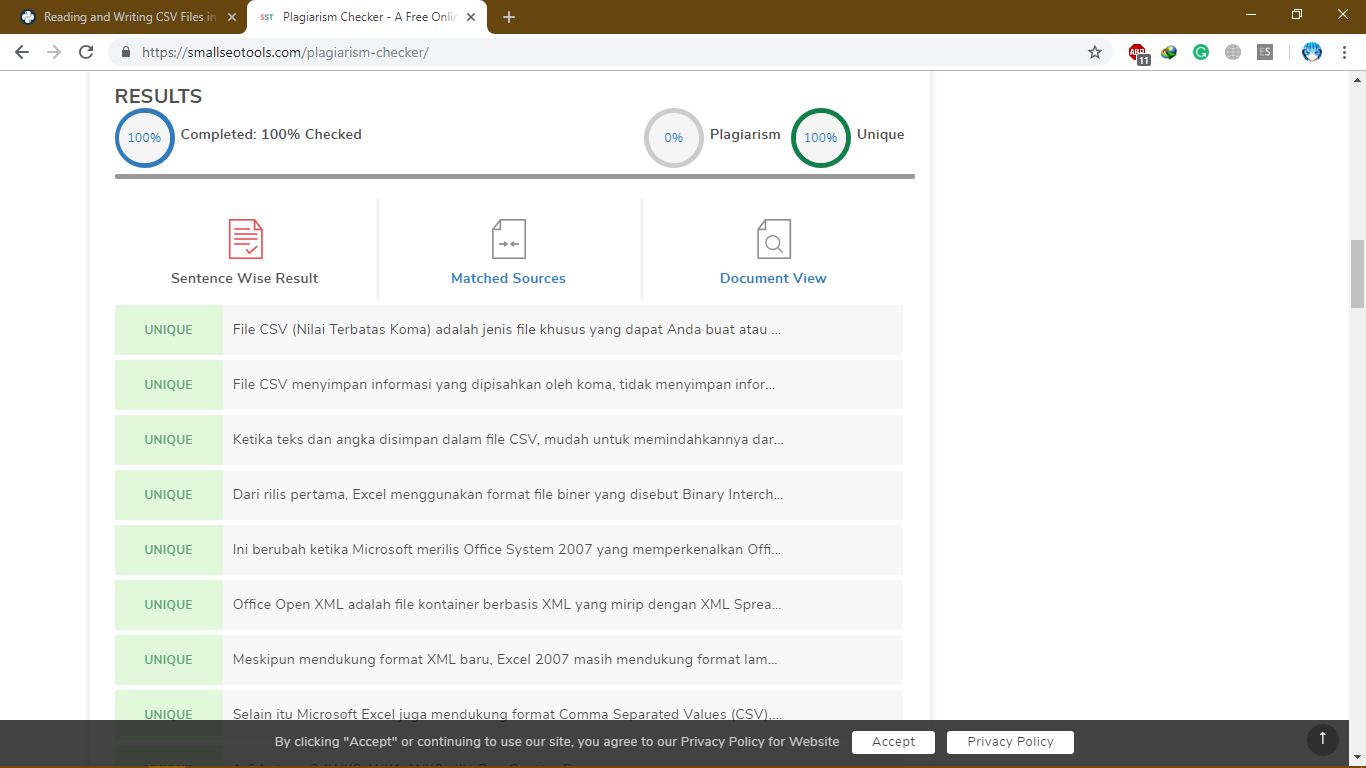
\includegraphics[width=10cm]{figures/4/1174027/teori/harunpla.png}
    \caption{SS Bebas Plagiarisme}
    \label{harun}
\end{figure}

\section{Sri Rahayu}
\subsection{Soal 1}
Isi jawaban soal ke-1

Kalau mau dibikin paragrap \textbf{cukup enter aja}, tidak usah pakai \verb|par| dsb

%\subsection{Soal 2}
%Isi jawaban soal ke-2

%\subsection{Soal 3}
%Isi jawaban soal ke-3

\section{Doli Jonviter}
\subsection{Soal 1}
Isi jawaban soal ke-1

Kalau mau dibikin paragrap \textbf{cukup enter aja}, tidak usah pakai \verb|par| dsb

%\subsection{Soal 2}
%Isi jawaban soal ke-2

%\subsection{Soal 3}
%Isi jawaban soal ke-3

\section{Rahmatul Ridha}
\subsection{Soal 1}
Isi jawaban soal ke-1

Kalau mau dibikin paragrap \textbf{cukup enter aja}, tidak usah pakai \verb|par| dsb

%\subsection{Soal 2}
%Isi jawaban soal ke-2

%\subsection{Soal 3}
%Isi jawaban soal ke-3

\section{Tomy Prawoto}
\subsection{Soal 1}
Isi jawaban soal ke-1

Kalau mau dibikin paragrap \textbf{cukup enter aja}, tidak usah pakai \verb|par| dsb

%\subsection{Soal 2}
%Isi jawaban soal ke-2

%\subsection{Soal 3}
%Isi jawaban soal ke-3
